
\section{\papername Decoding Flow and Architecture}

When using the 1D-chain matrix product state for decoding, directly enumerating all logical spins will incur exponential complexity with the number of logical qubits. Thus, we develop a partial tracing strategy to compute the conditional marginal probability of each logical spin in parallel. This strategy takes only $O(M\chi^2+\log K \cdot K^2\chi^4)$ with the number of syndrome checks $M$, the number of logical qubits $K$, and the virtual bond $\chi$  (the dimension of the matrix) of matrix product states, meanwhile maintaining the accuracy of decoding. Based on this polynomial-time decoding flow, we design a dedicated hardware architecture and implement it on the GPU device. We leverage the tensor core for matrix product and the CUDA core for calculating the marginal logical probabilities.

\subsection{Online Decoding via Conditional Marginal Probability}

The 1D-chain MPS contains the free energy under all syndromes and logical spin configurations. The decoding goal is to find the logical spin configuration with minimal free energy when given the syndrome spins. Directly enumerating all logical spin configurations needs $O(2^K(M+K)\chi^3)$, where $K$ is the number of logical qubits, $M$ is the number of syndrome qubits, and $\chi$ is the maximum virtual bond of the 1D-chain MPS.

To overcome the enumeration, we propose to calculate the marginal probability of each logical spin. The marginal probability is computed as 
\begin{equation}\small
    P(l_i=1|\vec{s}) = 
    \frac{{\text{contract}}(\mathcal{T}(l_i=1,\vec{s}))}{\text{contract}(\mathcal{T}(\vec{s}))}. 
    \label{}
\end{equation}
This means we only need to contract the 1D-chain MPS twice under the values of $g_i$ to get the marginal probability. However, using the marginal probability may not determine the value of logical spin $g_i$. For example, when the marginal probability is around 0.5, the value of logical spin can be 1 or -1 with the same probability. To find the most likely logical spin values, we further calculate their conditional probability under the determined spin values. 




\begin{figure}[t]
\centerline{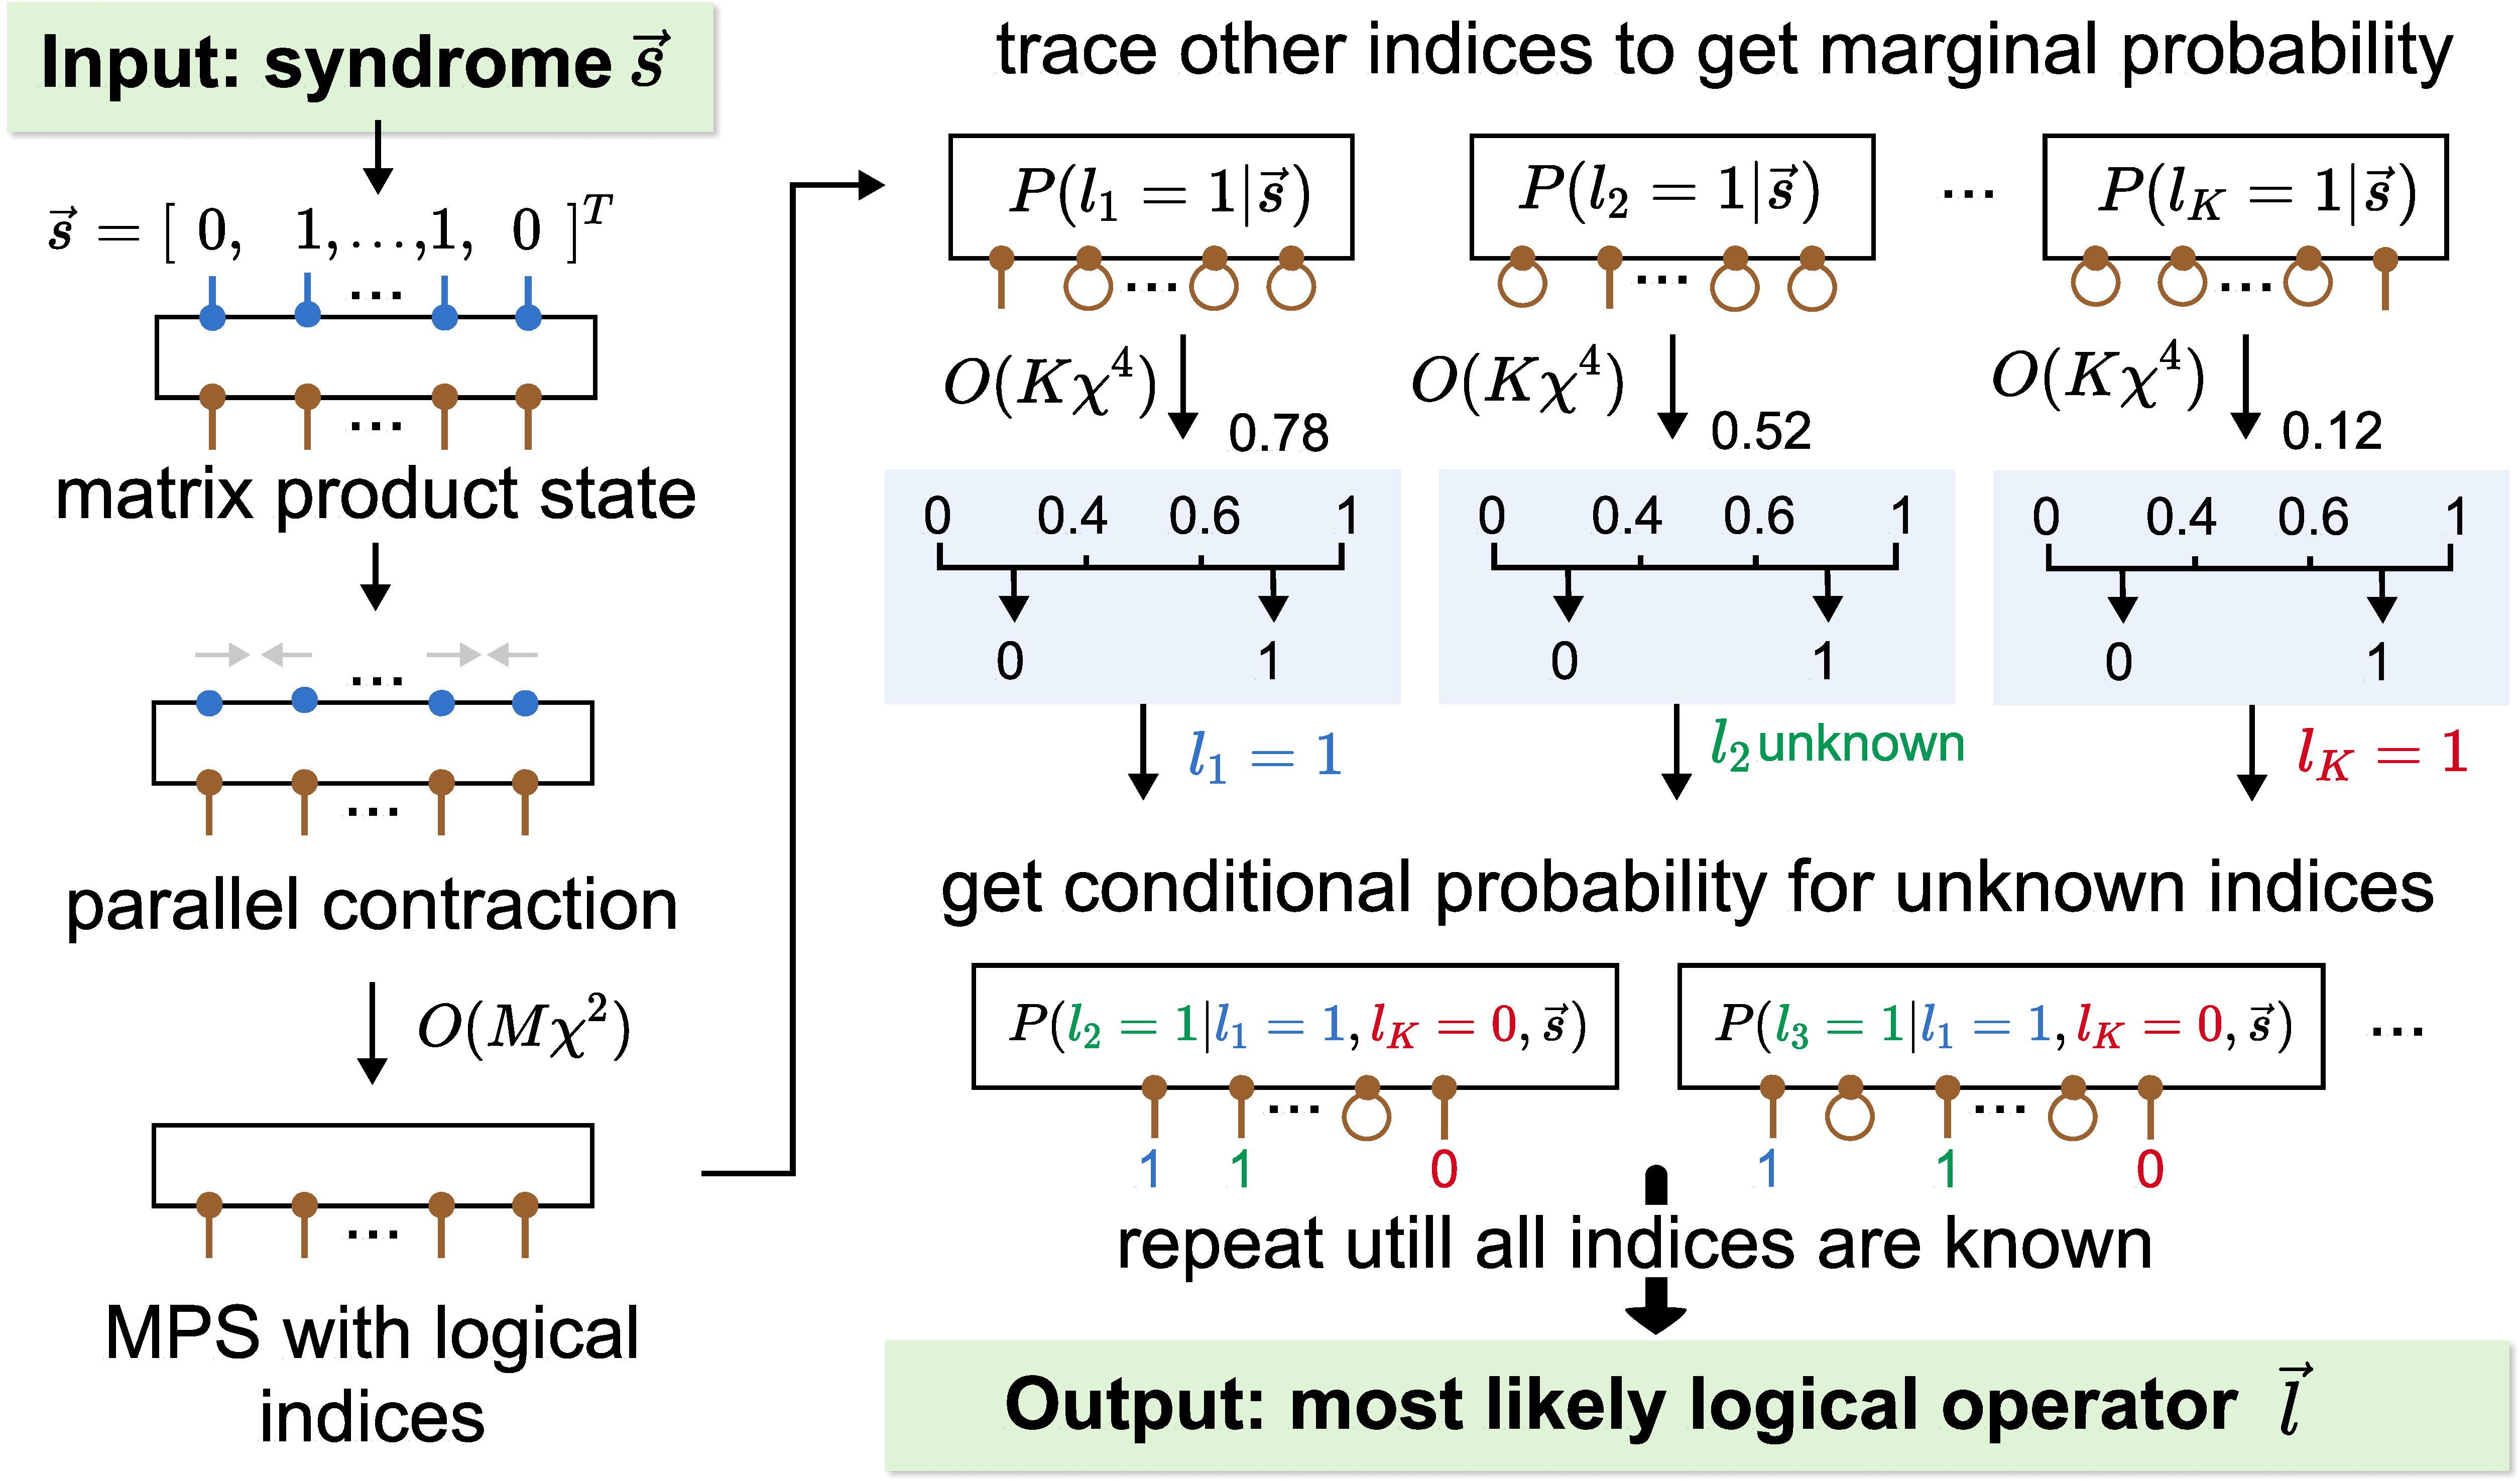
\includegraphics[width=0.98\columnwidth]{figures/logicaldecoding.pdf}}
\vspace{-0.2cm}
\caption{Online decoding via marginal probability calculation.} 
\vspace{-0.4cm}
\label{fig:decoding}
\end{figure}

\textbf{Online decoding flow and complexity analysis}.
\autoref{fig:decoding} illustrates the proposed online decoding flow. The decoder takes the measured syndrome vector $\vec{s}$ as input, representing the outcomes of stabilizer measurements. The MPS e
ncodes the free-energy landscape over all syndrome–logical spin configurations. Given $\vec{s}$, we contract the MPS to obtain one involving only logical spin indices, with a cost of $O(M\chi^2)$, where $M$ is the syndrome length and $\chi$ the maximum bond dimension. To determine the optimal logical spin configuration $\vec{l}$, the marginal probability of each logical spin $l_i$ is computed in parallel by tracing over other indices, requiring $O(K\chi^4)$ computation, where $K$ is the number of logical spins. Spins with probabilities close to 0 or 1 are fixed directly, while ambiguous ones (around 0.5) are refined through local conditional contractions, iterated $O(\log K)$ times. Finally, the recovered logical operator $\vec{l}$ is used to correct the physical state via the~\eqref{eq:recovererror}. This hierarchical contraction strategy reduces complexity from exhaustive enumeration to $O(M\chi^2+\log K\cdot K^2\chi^4)$ sequentially and $O(M\chi^2+\log K\cdot K\chi^4)$ in parallel, enabling scalable decoding.


\subsection{Hardware Architecture of Online Decoding}

\begin{figure}[t]
\centerline{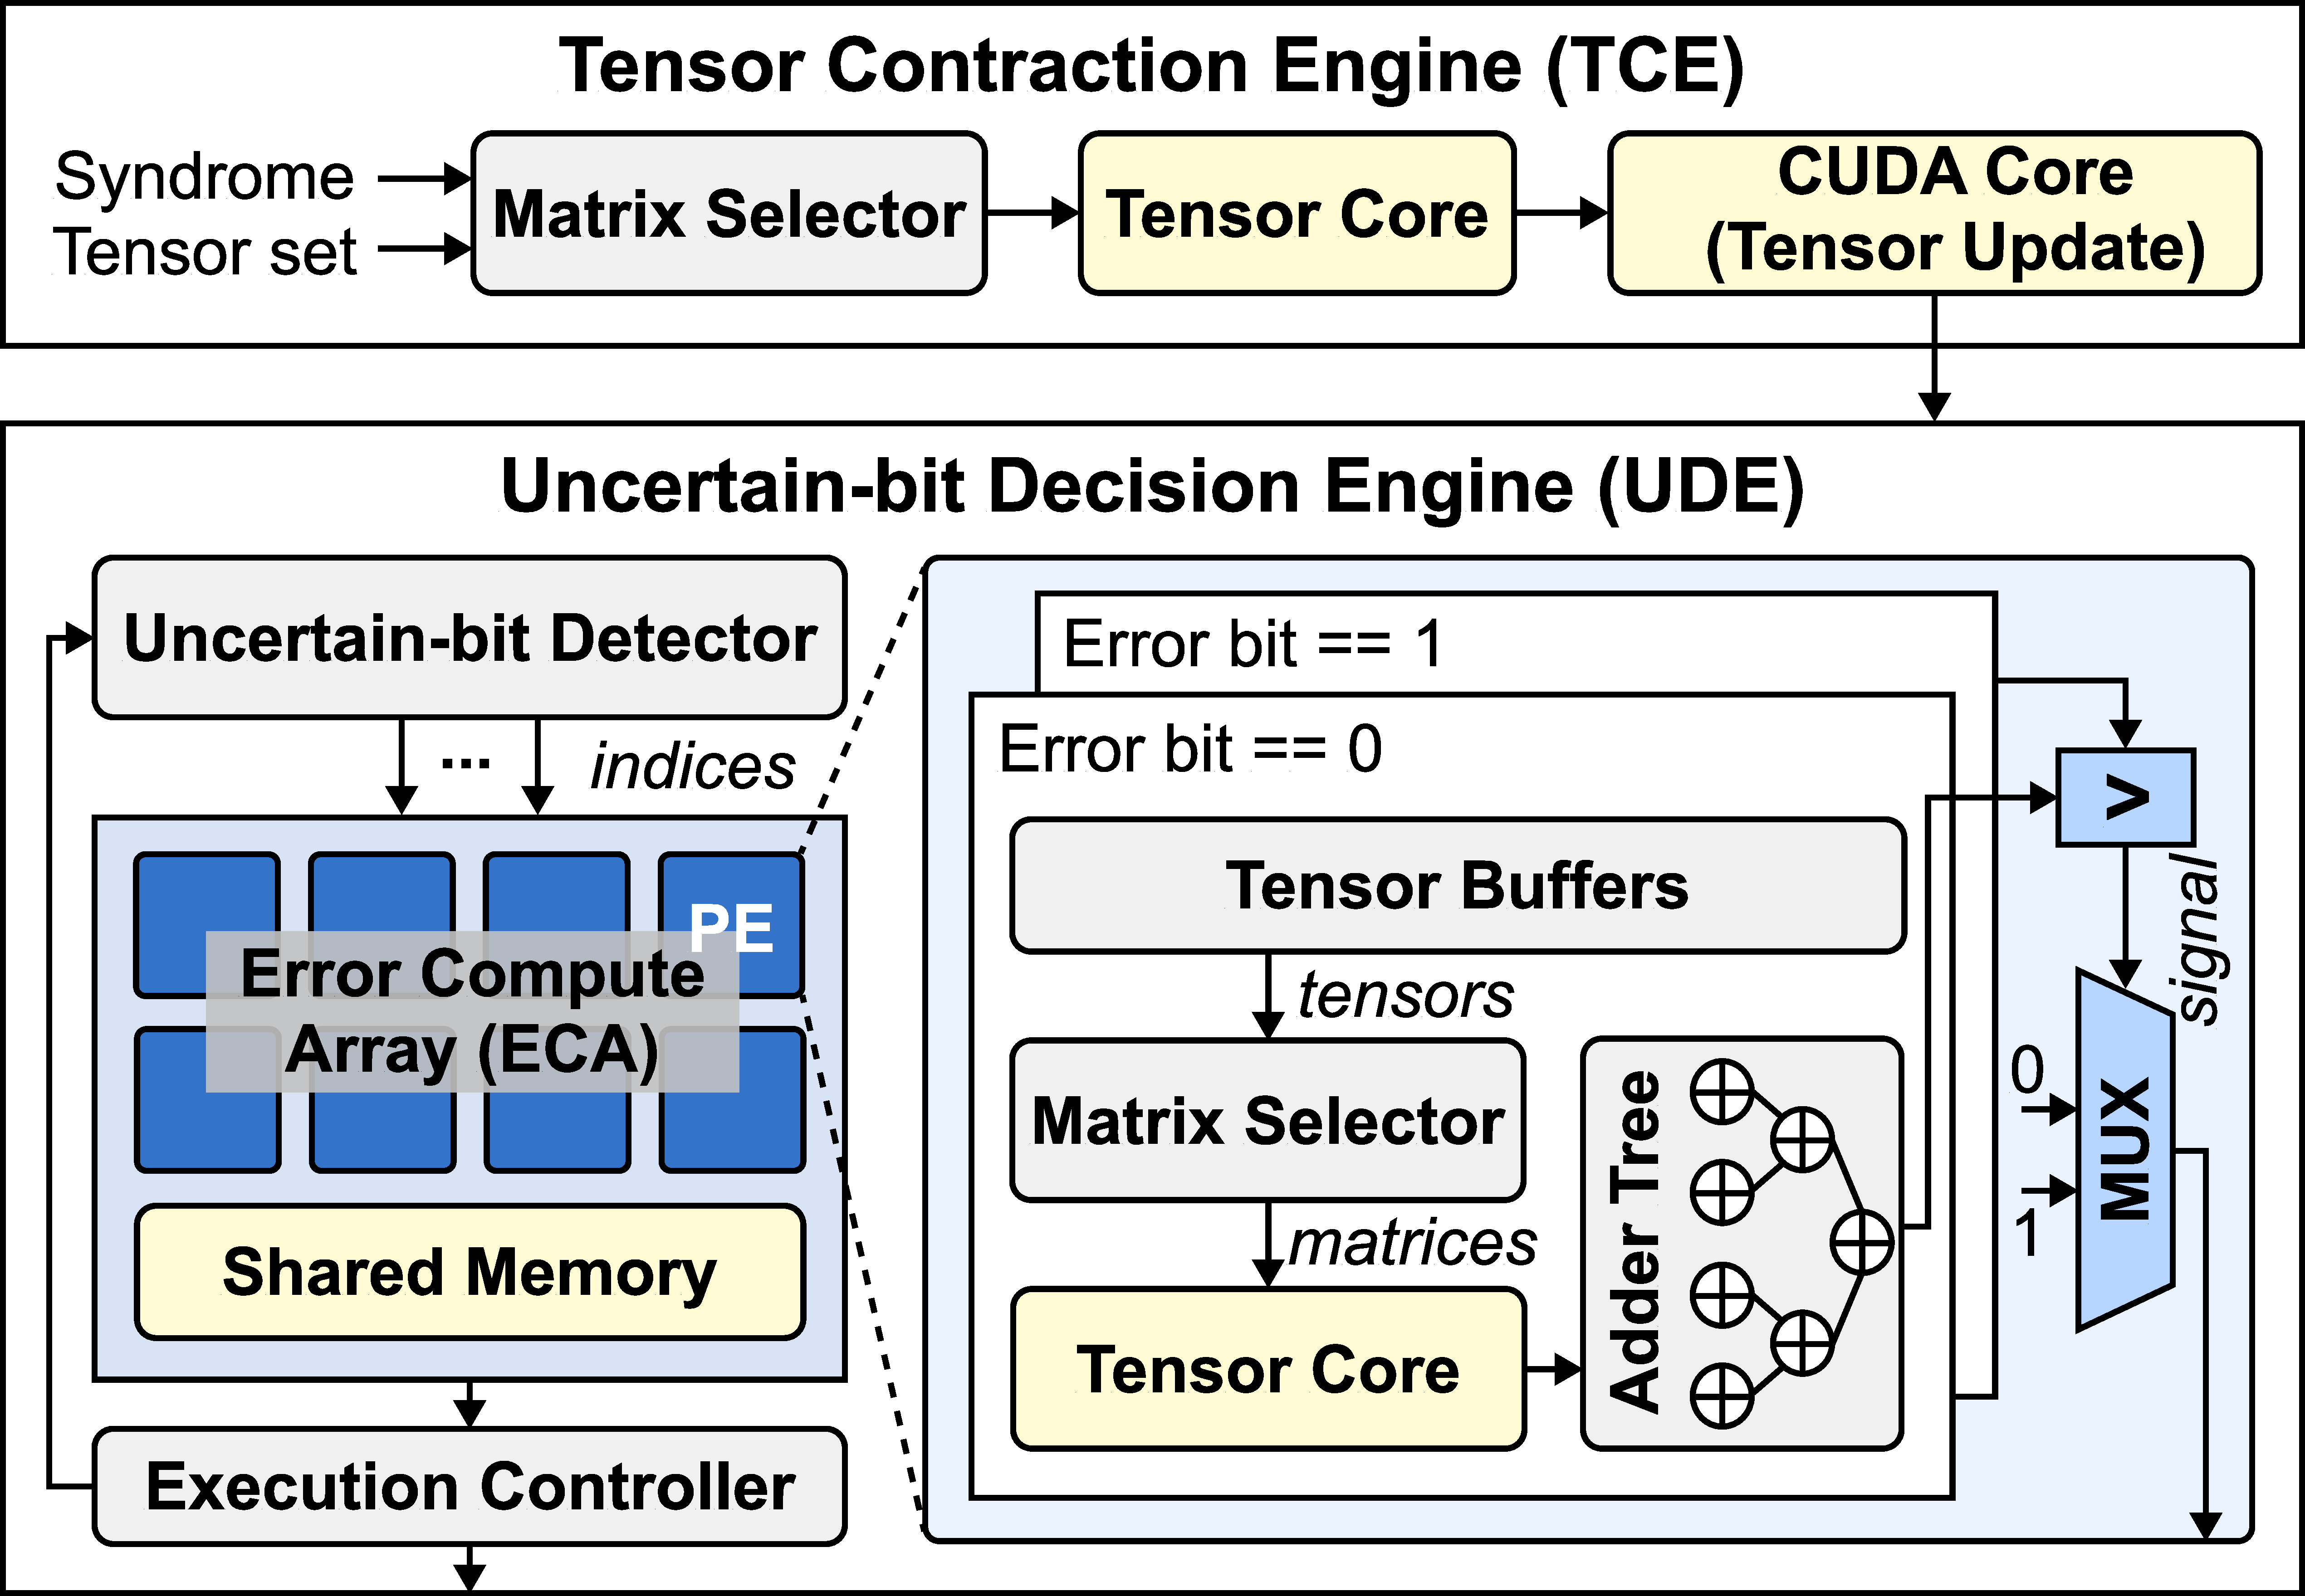
\includegraphics[width=0.95\columnwidth]{figures/gpu_hardware.pdf}}
\vspace{-0.2cm}
\caption{Hardware architecure support for \papername online decoding.} 
\vspace{-0.2cm}
\label{fig:gpu_hardware}
\end{figure}

\autoref{fig:gpu_hardware} presents the \papername hardware architecture designed to support the online decoding computational flow. The architecture consists of two major components: (1) a tensor contraction engine (TCE) and (2) an uncertain-bit decision engine (UDE). The TCE takes the syndrome and the tensor set as inputs. It leverages tensor cores to perform matrix multiplications in parallel and stores intermediate contraction results in shared memory to minimize global memory traffic during iterative tensor updates. A tensor update unit implemented using CUDA cores constructs the 1D-chain MPS with only $K$ tensors and writes them back to the on-chip tensor buffer. Once the MPS chain is generated, it is streamed to the UDE for determining the most probable logical spin configuration.

Within the UDE, an uncertain-bit detector identifies unknown logical indices whose marginal probabilities fall into the uncertainty and dispatches them to the error compute array (ECA). The ECA consists of multiple processing elements (PEs), each dedicated to resolving one uncertain bit. In each PE, the likelihoods for the spin value equal to 0 and 1 are computed in parallel. Specifically, a matrix selector first retrieves the relevant tensors from the on-chip tensor buffers (in shared memory) and feeds the selected matrices to tensor cores. The resulting matrix is then sent to an adder tree implemented by CUDA core–based parallel reductions, which accumulates its diagonal elements to compute the likelihood. Then, we compare the two likelihoods to determine the final value. All uncertain bits are processed in parallel across the PEs to maximize concurrency. Finally, an execution controller monitors whether unresolved bits remain in the logical operator $\vec{l}$. If so, it triggers another round of refinement; otherwise, the decoding process terminates.

% Looking forward, several stages of the pipeline can benefit from FPGA-based design. For example, the tensor update path in the TCE can be mapped to a fully pipelined contraction unit with a scratchpad hierarchy, removing the general-purpose overheads of tensor cores. Likewise, the uncertain-bit detector of UDE matches FPGA spatial parallelism: each PE can be implemented as a hardwired datapath with fixed matrix selection and reduction logic, enabling deterministic per-bit processing. In addition, a lightweight FPGA control engine can orchestrate refinement rounds without GPU scheduling overhead. With these customized modules, the end-to-end latency can be reduced substantially. For instance, a GPU-bound latency on the order of $10^3 \mu s$ can be decreased to sub-$10^1 \mu s$, yielding both higher throughput and better energy efficiency than a pure GPU design.